\chapter{Implementation}

\section{SSATools Package}
IRTools \cite{julia_irtools} is a similar existing tool to SSATools, but it uses an SSA IR completely separate from the existing compiler and is based on the lowered IR. The sub-functions used by IRTools and the lowered IR cannot be easily mapped to digital hardware control flow. Using the separate IR or the lowered IR would result in significant additional complexity in the later stages of the flow. The typed IR is the basis for the SSATools package, with the additional directive to avoid using a completely separate IR form.

The typed IR has a stricter SSA form than the IRTools package and the lowered IR, since it eliminates reliance on intermediary slot variables and provides explicit type and method choices for sub-functions. SSATools will be utilised as part of the HLS flow to extract the useful control and dataflow information from the compiled SSA structure. This package makes use of the existing reflection macro \code{@code\_typed} to expose the CodeInfo objects for user-defined, generic functions as well as the Julia compiler method \code{inflate\_ir} to extract the control flow graph. An example of the CodeInfo object returned from \code{@code\_typed} is in Code Snippet \ref{code:jpow_tir}.

%\subsection{\code{ci\_insert!} \& \code{ci\_delete!}}
\subsection{Typed IR/CodeInfo Manipulation}
There were no functions within the Julia compiler source code that could be easily exposed to the user that would allow the insertion and deletion of new SSA expression nodes within the CodeInfo object. So, a new function was created to be able to insert a Julia Expression at the specified position within the SSA code array. On the insertion of a new expression, the SSA values referenced within the rest of the code array are then updated to reflect the shift in the SSA values. This is necessary to preserve the connection between the index at which the expression is stored and the SSA value corresponding to the expression.

The first iteration of these functions produced incomplete CodeInfo objects that caused the Julia environment in which they were run to access illegal memory locations, resulting in segmentation faults. From the documentation, it was not clear which other members of the CodeInfo object needed to be updated. It was determined that the length of the \code{ssavaluetypes} and \code{ssaflags} arrays must match that of the array storing the lines of the IR. The insert function was then amended so that the type information of the expressions being inserted is insterted into the \code{ssavaluetypes} array at the same index of insertion as the expression, so that the new SSA value contains a type. All functions tested used a zero value in the \code{ssaflags} array, so the array was updated with an additional zero value on insertion. The current implementation of the Julia compiler states that these flags are currently reserved and not yet implemented \cite{ci_doc}, so this value will likely need to be changed in future versions if the core Julia compiler starts using the flags.

Code Snippet \ref{code:insert_ex} shows an example of the \code{ci\_insert!} being used to add a new line to the start of the simple power function with typed IR given in Code Snippet \ref{code:jpow_tir}. The new line will simply print a string, and is comprised of the \code{:call} symbol, the method reference \code{Base.println} and a string argument for the print function. The \code{@code\_typed} macro generates a Julia Pair containing the CodeInfo type at the first index and the return type at the second index. The expression is inserted into the CodeInfo object at the position of SSA value 1, producing the CodeInfo obect in Code Snippet \ref{code:insert_ci_res}.

\begin{lstlisting}[
caption={Example of using the \code{ci\_insert!} on the power function to insert a simple print statement.},
captionpos=b, 
label={code:insert_ex}
]
function jpow(x, n) #basic power function
        r = 1
        while n > 0
                n -= 1
                r *= x
        end
        return r
end

test_expr = Expr(:call, GlobalRef(Base, :println), "I am an SSA insertion")

pow_tir = @code_typed jpow(1,1)

SSATools.ci_insert!(pow_tir[1], 1, test_expr)

\end{lstlisting}

\begin{lstlisting}[
caption={Resulting CodeInfo object (representing typed IR) from the insert function in Code Snippet \ref{code:insert_ex}. SSA variable names were successfully incremented and control flow was preserved.},
captionpos=b, 
label={code:insert_ci_res}
]
CodeInfo(
1 -      Base.println("I am an SSA insertion")::Any
'--      nothing::Nothing
2 - %3 = phi (#1 => 1, #3 => %8)::Int64
|   %4 = phi (#1 => _3, #3 => %7)::Int64
|   %5 = Base.slt_int(0, %4)::Bool
'--      goto #4 if not %5
3 - %7 = Base.sub_int(%4, 1)::Int64
|   %8 = Base.mul_int(%3, x)::Int64
'--      goto #2
4 -      return %3
) => Int64
\end{lstlisting}

The final challenge of the insert function was the preservation of the links within the CFG (unless deliberately altered by the insertion of branching operations). The links within the CFG are implicit, based on the targets of the branch conditions and fall through of adjacent basic blocks. When an SSA expression is inserted at the position of the head of a basic block, the branches that target this position remain unchanged by the insert function. This maintains the control flow of the program. The current version of this function has been verified according to the existing unit tests. 

The solution for maintaining the control flow was carried over to the \code{ci\_delete!} function. However, the current delete performs an unavoidably more naive SSA reference correction returning a CodeInfo object that may error unexpectedly if a fundamental line in the SSA is removed. This results from the potential for remaining expressions to continue referencing the deleted SSA value. This could lead to incompatible types, alteration of the control flow or cause the Julia environment to crash. To prevent such errors, the \code{ci\_ssa\_replace!} method was added. This function iterates the expressions in the CodeInfo object and converts the target SSA value to the replacement SSA value. This method can be used in conjunction with \code{ci\_delete!} to make valid changes to the CodeInfo object. Though not currently part of the HLS flow, a typed IR pass was created to remove instances of the sign extension method (\code{Base.sext\_int}). This pass iterates over the CodeInfo object and collates the indices of the sign extension method. Each reference to these indices in the other expressions is replaced by the predecessor SSA value and the sign extension methods subsequently deleted. This pass and others based on the set of typed IR manipulation methods form the basis of the SSATools package for code manipulation.

\subsection{\code{ci\_to\_f}}
As part of the verification process, a successfully altered typed IR needs to be transformed back into a function that can be called by the user. The \code{ci\_to\_f} method takes as input a lowered or typed IR CodeInfo object and transforms it into an anonymous function. Due to the position in which the lowered IRs are produced in the compiler flow, the existing \code{@generated} macro can be used to generate anonymous functions without any alterations to the CodeInfo object (similar to IRTools \cite{julia_irtools}). For this case, the macro is attached to the CodeInfo object, evaluated and returned to the user.

\begin{figure}[htb!]
    \centering
    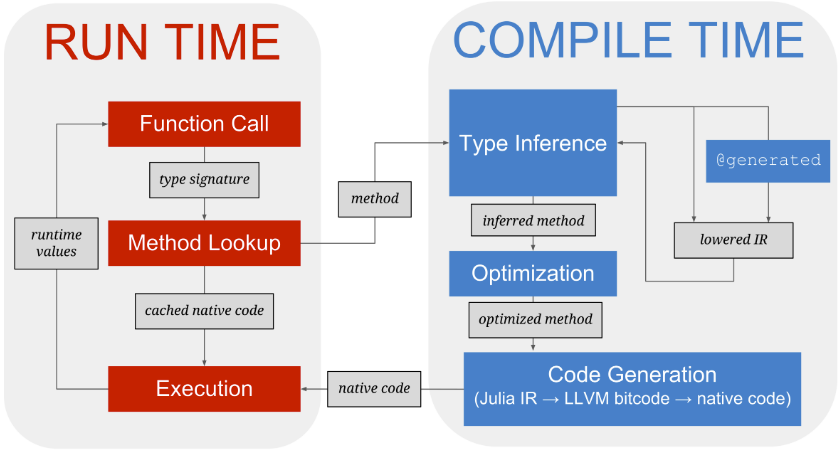
\includegraphics[width=0.8\textwidth]{Images/v2julia_compiler.png}
    \caption{Julia Compiler and Run-Time Flow \cite{julia_compiler_dia}}
    \label{fig:julia_compiler_flow}
\end{figure}

The final stages of type inference are completed after the macro expansion stage (\code{@generated}) as seen in Figure \ref{fig:julia_compiler_flow}, so the typed IR CodeInfo object needs to be transformed into the lowered IR before being used to generate anonymous functions.
 
\pagebreak

The \code{inferred} member of the CodeInfo object was thought to be a signal to the Julia compiler that a CodeInfo object had been through all iterations of type inference and would be used to determine the methods that would operate on the CodeInfo object to continue the compilation. Unfortunately, this member was just a flag and had no observable effect compiler's treatment of the CodeInfo object. The lowered and typed IRs of several functions were compared to determine the differences in the CodeInfo object. The first difference was in the CodeInfo object member: \code{ssavaluetypes}. The lowered IR contained an integer value matching the size of the array storing the expressions whereas the typed IR contained the types of each expression. Converting from an array of inferred types, to an integer the size of the code array caused the compiler to treat the CodeInfo object as if it were a lower IR. The conversion for the \code{jpow} example:\\ \code{pow\_tir[1].ssavaluetypes = Any[Any,Nothing,Int64,Int64,Bool,Any,Int64,Int64,Any,Any]}\\ is converted to \code{10}. 

This small change worked for simple functions but some CodeInfo objects contain expressions that are instances of invoked methods. This means that the expression head is the \code{:invoke} symbol rather than a \code{:call} symbol. Invoking a method allows the expression to use a particular version of a method without relying on multiple dispatch. Leaving these methods in causes the Julia environment to error. The solution to this issue was to convert these methods from the explicit method instances, chosen by type inference, to normal function calls with the input arguments associated with the invoked method instance. This may be unsafe due to specialisations performed as the anonymous function is re-run through type inference, but the current unit tests pass.

The lowered IR uses slot variables to store values that need to be reassigned as part of the control flow. The equivalent for slot variable reassignment in the typed IR are PhiNodes. These are special expressions within the typed IR that are used as part of the control flow. The basic block containing a PhiNode will have multiple predecessor blocks. For each predecessor, the result of the PhiNode will be a different SSA value. For example \code{\%3 = phi (\#1 => 1, \#3 => \%8)} states that the SSA value 3 is equal to the constant value 1 if the program has reached this block from basic block 1 and equal to SSA value 8 if the program came from basic block 3. PhiNodes are not used in the lowered IR, so their inclusion in the generated macro can inconsistently introduce errors in the resulting code due to over-zealous constant propagation in the compiler. Constant propagation reduces some or all of the PhiNodes expressions to compile time constants, disrupting the control flow of the program. To solve this issue a set of methods were created to convert PhiNodes into slot variables to produce a compatible lowered IR for anonymous function generation.

The IRTools package uses its own version of the Julia PhiNodes, so would be unable to return working anonymous functions with a direct translation to Julia IR. However, it contains custom evaluation function utilities \cite{julia_irtools_utils} to remove the IRTools PhiNodes and replace them with Julia's Lowered IR PhiNodes. The code inside the SSATools \code{rpl\_phinodes} function was created to operate on the typed IR to provide the same result as the IRTools evaluation functions. The result for \code{jpow} is in Code Snippet \ref{code:nophi}.

\pagebreak

\begin{lstlisting}[
    caption={Typed IR CodeInfo object of Code Snippet \ref{code:insert_ci_res} after PhiNode replacement.},
    captionpos=b, 
    label={code:nophi}
]
CodeInfo(
1 -      Base.println("I am an SSA intertion")::Any
|        (phi_2_1 = 1)::Any
|        (phi_2_2 = n@_3)::Any
'--      nothing::Nothing
2 - %5 = Base.slt_int(0, phi_2_2)::Bool
'--      goto #4 if not %5
3 - %7 = Base.sub_int(phi_2_2, 1)::Int64
|   %8 = Base.mul_int(phi_2_1, x)::Int64
|        (phi_2_1 = %8)::Any
|        (phi_2_2 = %7)::Any
'--      goto #2
4 -      return phi_2_1
)
\end{lstlisting}

The SSATools method \code{rpl\_phinodes} uses \code{ci\_insert!} to introduce additional slot variables that can be reassigned (unlike SSA variables) to carry out the function of PhiNodes. The function steps through each basic block and its successors in the CFG to make sure that the control flow is identical. The \code{ci\_delete!} is then used to remove all the PhiNodes. The resulting CodeInfo object then undergoes some further minor transformations to make sure the remaining fields are the correct size before being returned as an anonymous function with the number of arguments specified by "\code{Nargs}". The example in Code Snippet \ref{code:cif_call} shows the result of calling the \code{ci\_to\_f} function on the altered typed IR from Code Snippet \ref{code:insert_ci_res} with the changes introduced in Code Snippet \ref{code:nophi}.

\begin{lstlisting}[
    caption={Use of \code{ci\_to\_f} to create an anonymous function. Use of the anonymous function to demonstrate typed IR alterations.},
    captionpos=b, 
    label={code:cif_call}
]

ff = SSATools.ci_to_f(pow_tir, 2)

julia> ff(2,3)
I am an SSA intertion
8
\end{lstlisting}

\subsection{\code{fcgraph}}
A Function Call Graph (FCG) represents all the sub-functions called from within the chosen function. \\ \code{fcg\_graph(function, arg\_types...)} generates this graph from the typed IR of a given function. This function depends on the LightGraphs \cite{julia_lightgrph} and MetaGraphs \cite{julia_metagrph} packages to produce, maintain and plot the directed graph structure as in Figure \ref{fig:mvfcg}. This function is required to decompose non-Base functions into Base functions.

\begin{figure}[htb!]
    \centering
    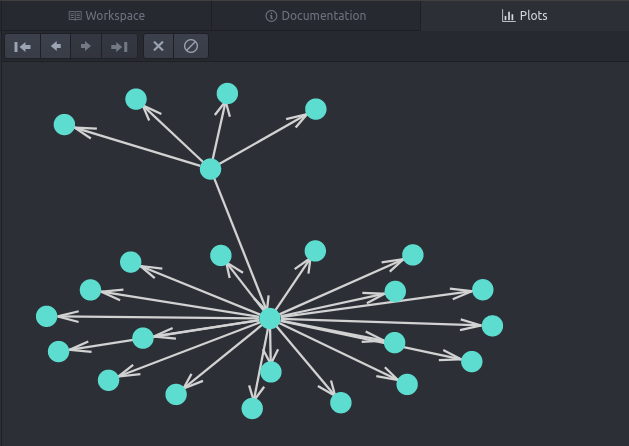
\includegraphics[width=0.6\textwidth]{Images/mv_fcg.png}
    \caption{Function Call Graph for the Matrix-Vector Multiply function in Code Snippet \ref{code:mv_mult}}
    \label{fig:mvfcg}
\end{figure}

\pagebreak

The function iterates through all the lines of code and pulls out the sub-functions, keeping track of the ones seen before. These are added as nodes directed from the "Main" node. If the function encounters a sub-function call that is not within Julia's "Base" code library, this is transformed into a global reference to the function and then expanded using \code{code\_typed}. The functions that branch from this expanded function are directed from the sub-functions node rather than "Main". All non-Base sub-function calls are broken down recursively to produce the full FCG. The MetaGraphs library is used to attach a dictionary containing the sub-function name and additional data about the sub-function to each node.

%TODO actually reference the mv mult

\begin{lstlisting}[
    caption={A simple example function to perform Matrix-Vector multiplications and the CodeInfo object for the function's typed IR.},
    captionpos=b, 
    label={code:mv_mult}
]
m_v_mult(M::AbstractMatrix{Int64}, v::AbstractVector{Int64}) = M*v

CodeInfo(
1 - %1 = Base.arraysize(M, 1)::Int64
|        Base.arraysize(M, 2)::Int64
|   %3 = Base.slt_int(%1, globalref.0)::Bool
|   %4 = Base.ifelse(%3, 0, %1)::Int64
|   %5 = $(Expr(:foreigncall, :(:jl_alloc_array_1d), 
		Array{Int64,1}, svec(Any, Int64), :(:ccall), 2, 
		Array{Int64,1}, :(%4), :(%4)))::Array{Int64,1}
|   %6 = invoke LinearAlgebra.generic_matvecmul!
		(%5::Array{Int64,1}, 'N'::Char, _2::Array{Int64,2}, 
		_3::Array{Int64,1})::Array{Int64,1}
'--      return %6
) => Array{Int64,1}
\end{lstlisting}



\pagebreak

\begin{lstlisting}[
    caption={The metagraph data stored at each node in the FCG for the Matrix-Vector multiplication example.},
    captionpos=b, 
    label={code:fcg_dict}
]
#The top level sub-functions inside the main function
(:Type => Int64,:Func => :(Base.arraysize),:Head => :call,:Level => 2)
(:Type => Bool,:Func => :(Base.slt_int),:Head => :call,:Level => 2)
(:Type => Int64,:Func => :(Base.ifelse),:Head => :call,:Level => 2)
(:Type => Array{Int64,1},:Func => :(:jl_alloc_array_1d),:Head => :foreigncall,:Level => 2)
(:Type => Array{Int64,1},:Func => :(LinearAlgebra.generic_matvecmul!),:Head => :invoke,:Level => 2)

#The functions contained within the :(LinearAlgebra.generic_matvecmul!)
(:Type => Int64,:Func => :(Base.arraysize),:Head => :call,:Level => 3)
(:Type => Bool,:Func => :(Base.or_int),:Head => :call,:Level => 3)
(:Type => Bool,:Func => :(Base.not_int),:Head => :call,:Level => 3)
(:Type => ArgumentError,:Func => :(Core.ArgumentError),:Head => :new,:Level => 3)
(:Type => Union{},:Func => :(Base.throw),:Head => :call,:Level => 3)
(:Type => Int64,:Func => :(Base.arraylen),:Head => :call,:Level => 3)
(:Type => UInt32,:Func => :(Base.bitcast),:Head => :call,:Level => 3)
(:Type => String,:Func => :(Base.print_to_string),:Head => :invoke,:Level => 3)
(:Type => DimensionMismatch,:Func => :(Base.DimensionMismatch),:Head => :new,:Level => 3)
(:Type => Union{},:Func => :(LinearAlgebra.throw),:Head => :call,:Level => 3)
(:Type => Bool,:Func => :(Base.sle_int),:Head => :call,:Level => 3)
(:Type => Int64,:Func => :(Base.ifelse),:Head => :call,:Level => 3)
(:Type => Bool,:Func => :(Base.slt_int),:Head => :call,:Level => 3)
(:Type => Int64,:Func => :(Base.sub_int),:Head => :call,:Level => 3)
(:Type => Int64,:Func => :(Base.mul_int),:Head => :call,:Level => 3)
(:Type => Int64,:Func => :(Base.add_int),:Head => :call,:Level => 3)
(:Type => Int64,:Func => :(Base.arrayref),:Head => :call,:Level => 3)
(:Type => Array{Int64,1},:Func => :(Base.arrayset),:Head => :call,:Level => 3)
\end{lstlisting}

Node information can be viewed using the SSATools function \code{printfcg\_vdict}, giving the output shown in Code Snippet \ref{code:fcg_dict}. Each dictionary contains:
\begin{itemize}
\item The type of the SSA variable.
\item The sub-function called at that SSA code line.
\item The expression head dictating the type of call.
\item The depth level the sub-function is within the main function.
\end{itemize}

\pagebreak

The main challenge with this function was how to decompose the non-Base methods such as the\\ \code{LinearAlgebra} method in Code Snippet \ref{code:mv_mult}. The only way to obtain the Base operations of non-builtin functions is to use the reflection tools. The \code{@code\_typed} macro can produce the IR from a function call, so we thought it was possible to directly use the expression with the macro. This failed as the SSA values and Slot variables were not themselves the correct type for the method. Instead, the \code{code\_typed} function can use a global reference to the method in addition to the types of the arguments required by the method to generate the same typed IR as the reflection macro, since they make use of the same underlying reflection methods.

The information provided in the CodeInfo object was enough to be able to use the \code{code\_typed} function. The method global reference is obtained from the second argument for standard function calls and the third argument for invoked methods. This is converted into a call by a helper function. The helper function extracts the method name from the global reference by obtaining the string representation, parsing it using the Julia Meta library, and then evaluating it to a direct function call.

The arguments in the method expression after the method name are the arguments to the method itself. These can be constant values, SSA values or Slot variables. The type of the constants is determined by the \code{typeof} Julia function and the type of the SSA values is determined by looking up the SSA index in the \code{ssavaluetypes} array. Similarly, the type of the Slot variable is determined by looking up the index of the Slot index in the \code{slottypes} field of the CodeInfo object. The function call and the input types become the arguments for the next recursion of the \code{fcgraph} function. The number of arguments passed to \code{fcgraph} is dependent on the methods being expanded, and will be converted to a Tuple for the \code{code\_typed} function. A tuple is an immutable structure so cannot be appended like a vector. Instead, we implemented the quote node from Julia's meta-programming system to automatically generate a Tuple with the desired types. This node is then evaluated and passed to \code{code\_typed} to continue generating the FCG.

\pagebreak

\subsection{Control Data Flow Graph (CDFG)}
Figure \ref{fig:cfg_pow} is diagram of the CFG of the example power function. The edges between the basic blocks are directed so the control and loops are obvious from these connections. The flow of data can be extracted from the links between SSA values but each expression only contains information about the predecessor values. The \code{Core.Compiler.inflate\_ir(CodeInfo)} function converts a CodeInfo object into an alternative IR object. This object contains CFG blocks which explicitly list control information that was implied in the CodeInfo object. The CFG blocks contain all the SSA expressions within the block as well as the predecessor and successor blocks. It also contains the CFG links in an array form. This does not contain all the necessary information for scheduling as the data dependencies are not represented. To associate the SSA values with their control flow, the basic block statements need to be searched each time. This makes the CFG alone a sub-optimal method to act as the interface to the later stages of the HLS flow.

\begin{figure}[htb!]
    \centering
    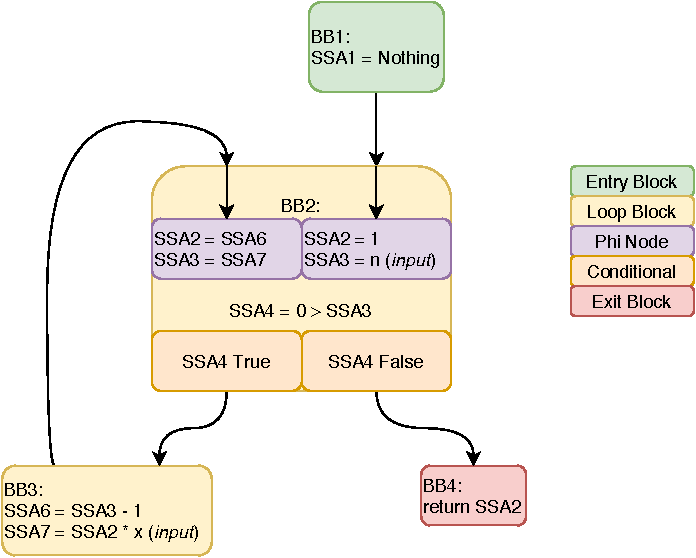
\includegraphics[width=0.6\textwidth]{Images/CFG.pdf}
    \caption{Control flow graph corresponding to the Typed Intermediate Representation of the pow function.}
    \label{fig:cfg_pow}
\end{figure}

The CDFG was chosen as the interface between the typed IR and the scheduling methods in the HLS flow based on existing tools \cite{legup_intro}, \cite{nymble_intro}. These papers show that the CDFG is an effective formal representation to store the program information required for scheduling. %The implementation of the CDFG is as follows.

\pagebreak

\begin{lstlisting}[
    caption={The CDFG node types containing the information extracted from the typed IR.},
    captionpos=b, 
    label={code:CDFG_types}
]
struct CDFGNode
    op::Any #operation
    bb::Int #basic block number
    type::DataType #type of data output by node

    dataPreds::Array{Array{T,1} where T, 1} # [ssa val (int) or constant, type, position, literal or not(boolean)]
    dataSuccs::Vector{Int} # [ssa val]
    ctrlPreds::Vector{Int} #control info, basic blocks
    ctrlSuccs::Vector{Int}
end

struct CDFGArg
    name::Symbol
    slotNum::Int
    type::DataType

    dataSuccs::Vector{Int} # [ssa val]
    ctrlSuccs::Vector{Int} 
end
\end{lstlisting}

The structure consists of three members: the CDFGArg (argument) array, the CDFGNode array and a copy of the CFG. The members of the CDFG custom types are shown in Code Snippet \ref{code:CDFG_types} with the CDFG connections represented in Figure \ref{fig:cdfg_pow}.

\begin{itemize}
	\item \textbf{op:} The operation associated with the node. For Julia Base expressions this is a global reference. These can be mapped directly to function operations in hardware. Symbols representing the phi nodes, branches and null expressions are also included in the operation, as this makes it easier to distinguish control flow from data manipulation.
	\item \textbf{bb:} The basic block in which the expression associated with the node is contained.
	\item \textbf{type:} The type of the SSA value that results from computing the expression associated with the node. If the operation is control flow or null, the type is generalised to \code{Any} type.
	\item \textbf{dataPreds:} A set of four arrays containing complete information about the dataflow predecessors for the node. The first contains the SSA values or constants, the second contains the types of these values, the third contains the position of the predecessors within the expression arguments and the fourth contains a boolean flag indicating whether or not the value is a constant or an SSA value (true means constant).
	\item \textbf{dataSuccs:} An array of the SSA values that the data from this node feeds in to.
	\item \textbf{ctrlPreds:} An array of the SSA values/basic blocks values that precede this SSA value/basic blocks.
	\item \textbf{ctrlSuccs:} An array of the SSA values/basic blocks values that follow on from this SSA value/basic blocks.
\end{itemize}

\pagebreak

\begin{figure}[htb!]
    \centering
    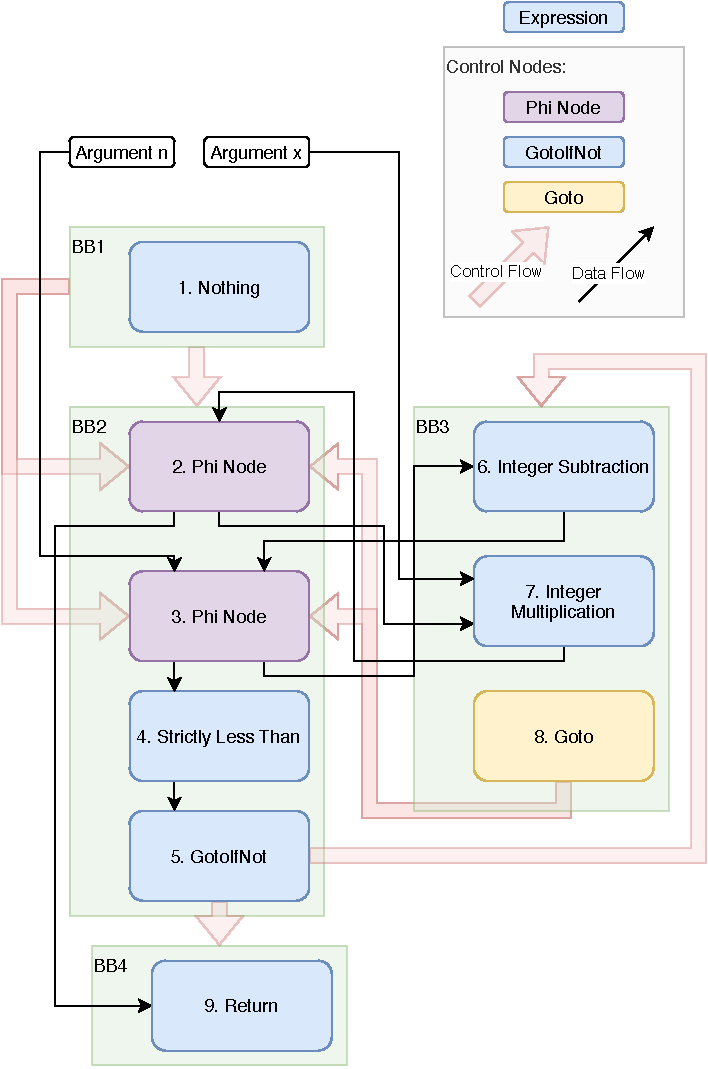
\includegraphics[width=0.6\textwidth]{Images/CDFG.pdf}
    \caption{Control Data Flow Graph generated from the Typed IR of the jpow function.}
    \label{fig:cdfg_pow}
\end{figure}

The main types within the CodeInfo object are \code{Expr}, \code{PhiNode}, \code{GotoNode} and the null type \code{Nothing}. Each type needs to be processed differently based on their internal fields. Multiple dispatch is used to simplify the CDFG generation function. Each line in the CodeInfo object can be passed as the line argument for the same function name. The \code{Expr} type contains the \code{:gotoifnot} and \code{:return} expressions that are handled differently to the expressions as they have a fixed number of arguments to be processed. There is currently no support for Julia  generator expressions (in-line for loops), as they reference methods stored in the main Julia environment that cannot currently be accessed from the CodeInfo object. The \code{Nothing} code lines cannot be ignored as these represent control flow placeholders for basic blocks with no operations. 

To reduce the number of passes of the CodeInfo expressions, the data predecessors and control predecessors are determined in the first run. The successors are determined from the predecessors to link CDFGNodes like a doubly-linked list. Both the predecessors and successors are needed, since the scheduling code relies on having forward and backward linking information. This information is available in $O(m)$ time, where $m$ is the number of predecessors/successors. This is faster than iterating through the full list of CDFG nodes, since there are  guaranteed to be more than $m$ nodes.

\pagebreak

\section{Dynamic Scheduling Package}
This package is responsible for generating functionally correct elastic circuits using a series of passes that dynamically schedule the CDFG. The output of this package is a DOT graph to be passed to the dynamatic library's VHDL converter \cite{dtv}.

\subsection{Elastic Circuit Types}

\iffalse
key design choice influenced by language - justify
	why have a million types
	method inference
	only need to add code
	dont need to amend if statements
	just add new tyeps and functions corresponding to those types
	
	many of the printing functions ended up being similar - to reduce boiler plate code
		got to make use of auto code gen
\fi

Figure \ref{fig:ec_types} shows a breakdown of the types used in the Dynamic Scheduling package. The Elastic Circuit type contains two vectors, the first of which contains an array of Elastic Components. Each Elastic Component corresponds to an equivalent component provided by the dynamatic library in VHDL. This library is derived from exisitng elastic component architectures in \cite{elastic_cgra}, \cite{elastic_sync}. The decision to use multiple, distinct concrete types was made to take advantage of multiple dispatch and support future code additions. When supporting a new operation, the developer would not be required to alter the existing functions. The code has added to the \code{Base.show} methods to print out the Elastic Circuit. In this DOT print, the print method is dispatched based on the component type. This allows the print function to have the same name and prevents the use of a large conditional statement. The developer would need to add a new concrete type, a print function for the component, and a print function for the links. The rest is handled by multiple dispatch.

Many of the types are constructed with similar inputs and outputs. To reduce the amount of boiler-plate code, a macro was created to automatically generate some of the print functions based on the type provided. 
		
\begin{figure}[htb!]
    \centering
    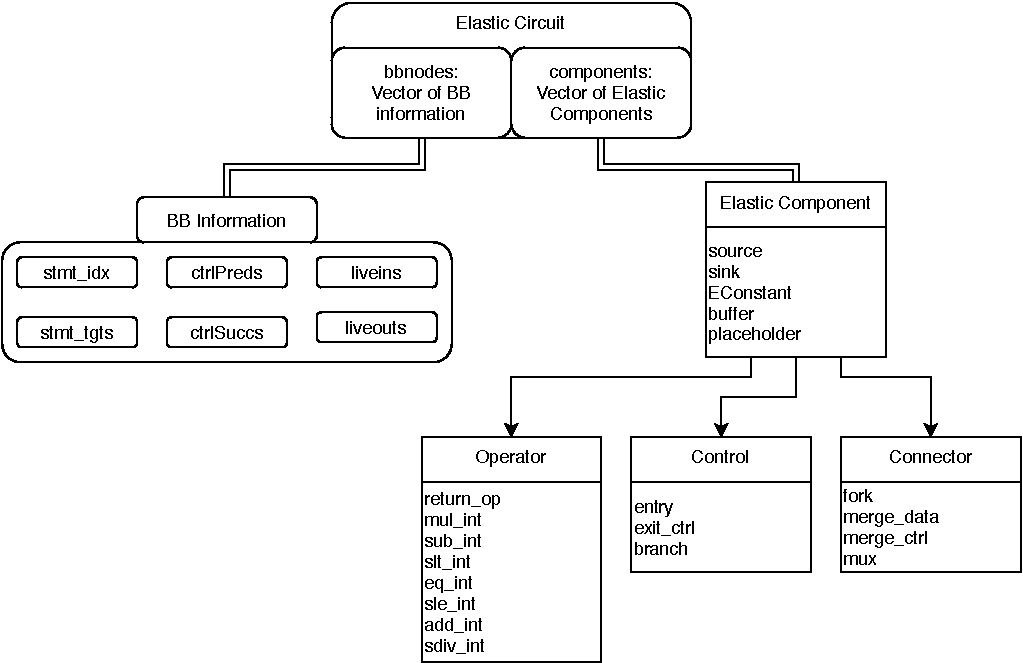
\includegraphics[width=\textwidth]{Images/ec_types.pdf}
    \caption{Elastic Circuit type breakdown. }
    \label{fig:ec_types}
\end{figure}

The BB information is constructed using dictionaries since this contains control information and does not need to be printed. The \code{stmt\_idx} is a list of integers representing the SSA values for the operations defined within the basic block. The \code{stmt\_tgts} is another dictionary containing the successors (and their basic blocks) for the operations defined within the basic block. The \code{ctrlPreds} and \code{ctrlSuccs} list the basic blocks linking to and from the current basic block.  A \code{livein} is an expression used within the current basic block that originates from a different block and a \code{liveout} is used outside of the current basic block. This information is used to determine where to add components when generating the elastic circuit. The dictionary data structure was chosen to make the code more readable as each member is reference by name rather than index.

%\subsection{Elastic Circuit Passes}
\iffalse
passes:
initial CDFG conversion
	first version didnt capture nothing cdfgnodes or goto statements
	design decision made for the branching statments to be initialised as control components
	components are effectively chanined together, you now have components connected across blocks
	the nature of dynamic scheduling means that only the components within the control path will be activated
	meaning that if a branching condition is not activated because its false rather than true, a basic block will not be branched to
	subsequent references to ssa values in that block will not be activated and the hardware won't function as intended

this is related to the global nature of SSA values
		fundamental difference between memory mapping in a program and the dynamic scheduling
		there's no global memory that can be accessed by all components
		so needed to implement a way of linking the definition of a given ssa value
		
		first you need to know the definition points for a value and each subsequent value it was used
		within a basic block, the value can just be connected as the order of operations in a basic block is sequential
		however if the value is defined in a different block you need to map a path from the definition block to each of its uses in other blocks
	the dynamatics tool uses liveness analysis to determine the nodes in need of connecting
	
liveness analysis 
	algorithm for determining live ins/outs
	
at the end of phi nodes, the liveouts and stmt idxs are updated with the phi nodes. so that the branches work
\fi
%TODO maybe explain why it works on index
\subsection{Initial Elastic Circuit Pass}
The intial pass iterates over the CDFG and pushes the component associated with the CDFG node operation to the list of components. For each component, the \code{stmt\_tgts} are updated with the successor information. The pass then iterates over the arguments and pushes \code{entry} types for each of the arguments. The first version of the initial pass added the arguments first and then the nodes which caused all of the predecessor and successor information to be made incorrect as this is based on array index. The dynamatics tool adds control components after the many of the passes have been run. Using the typed IR instead of LLVM allows this pass add control branches for the goto and gotoifnot CDFG nodes. After this initial pass, the components are chained together in the Elastic Component array. Even for simple functions, there will likely be many connections across basic blocks. The nature of dynamic scheduling means that only components within the active control path will have valid information. If a branching condition is not activated a successor basic block may never be reached and all subsequent references to the expressions within that block will not be active and the hardware will not function as intended.

This is related to the global nature of the SSA values within the typed IR. The fundamental difference between the SSA form and the dynamically scheduled form is the lack of access to global, monolithic memory. Additional components need to be added to the circuit to make sure that the references to component in which the value is defined and all successors are linked with respect to control flow. This is partially accomplished by the Phi Insertion Pass.

\subsection{Merge (Phi) Insertion Pass}
The pass starts by determining the definition points for each of the values. This is trivially taken from the \code{stmt\_idx} lists in the BB information. The pass then determines in which basic block the expressions are used. A use within the same basic block as the definition can just be connected because the order of operations within a basic block remains sequential. If the value is defined in a different block, a chain of components needs to be added through the intermediary basic blocks to link the definition and use. 

\begin{algorithm}[h]
\SetAlgoLined
\KwResult{List of live-in expressions for each basic block: bb\_live\_ins}
	bbnodes = BB Information\;
	bb\_definitions = Array of expressions indexed by basic block\;
	bb\_uses = Array of expression usages indexed by basic block\;
	
	bb\_live\_ins = [[], [], ...] array for each basic block\;
 	mod\_flag = true\;
 	\While{While mod\_flag}{
		mod\_flag = false\;
		
		\For{For \textbf{basic\_block} in bbnodes}{
			liveouts = []\;
			
			\For{For \textit{successor} in \textbf{basic\_block}["ctrlSuccs"]}{
				set\_union(liveouts, bb\_live\_ins[successor])\;
			}
			
			diff = set\_difference(liveouts, bb\_definitions[\textbf{basic\_block}])\;
			tmp = return\_set\_union(bb\_uses[\textbf{basic\_block}], diff)\;

  			\If{length(tmp) $>$ length(bb\_live\_ins[\textbf{basic\_block}])}{
   				bb\_live\_ins[\textbf{basic\_block}] = tmp\;
   				mod\_flag = true\;
   			}
		}
 	}

\caption{Algorithm to perform dataflow analysis \cite{liveness}.}
\label{alg:liveness}
\end{algorithm}

Algorithm \ref{alg:liveness} is used to determine the "liveness" of an expression (live-in or live-out). The final result is an array of live-ins for each basic block. Each block definition follows a chain of the live-ins to the uses in successor blocks. These values are then converted into merging nodes and the connections for definitions and uses altered to pass through the merging nodes.   This creates the data flow paths so that global memory references are no longer used.

\subsection{Branch Insertion Pass}
The merging nodes take one or more input connection but do not influence the control flow. The control branches do influence the flow of the circuit but each data point is connected to a series of merges which would all activate regardless of the flow. The branch pass introduces non-control branches for each of the variables that flow out of the basic block. These branches are required to have the same successors as the control branches as well as the same conditional expression to switch between the true and false branches. 

Each pass introduces more components to the circuit so looping over the components within the passes should be minimised. To aid this, the observation was made that, for simple functions, the last expressions in the \code{stmt\_idx} array of the BB information is always a control branch. This means that the pass doesn't have to search for the control branch for a given basic block when adding the branching targets and conditional statement. The assumption remained valid until testing a function with an implicit fall-through between basic blocks (as in Code Snippet \ref{code:imp_fall}). This is a product of using the typed IR which does not always use an expression to represent the end of a basic block. A block with a fall-through always transitions to next adjacent block (e.g. BB4 to BB5) but does not contain a branch meaning the assumption that the final value in the \code{stmt\_idx} is not always a control branch. 

\begin{lstlisting}[
    caption={Example of implicit fall through from BB4 to BB5. There is no control branch.},
    captionpos=b, 
    label={code:imp_fall}
]
3 - %6 = Base.slt_int(a, b)::Bool
'--      goto #5 if not %6
4 - %8 = Base.mul_int(%1, b)::Int32
5 - %9 = phi (#2 => %4, #4 => %8, #3 => %1)::Int32
\end{lstlisting}

The issue was resolved by including a check of the type of the last element in the \code{stm\_idx}. If the value is not a control branch, it can be assumed that one does not exist so the pass adds one driven by a constant value. This constant is then used as the conditional for the data branches generated by the pass.

The next assumption made was that each expression is only used at one point in successor basic blocks. Again this works for simple functions but the introduction of typed IR PhiNodes (elastic circuit multiplexers) means that an expression can be used as input to more than one multiplexer (see Figure \ref{fig:multi_mux}). The multiplexer is a merging node with a select line driven by the control components and a single branch is not allowed to attach to more than one merge. 

\begin{figure}[htb!]
    \centering
    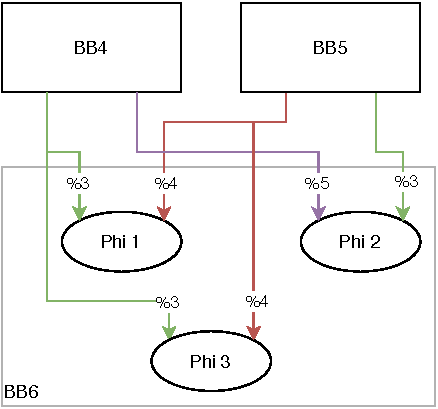
\includegraphics[width=0.4\textwidth]{Images/multi_mux.pdf}
    \caption{Diagram of more than one multiplexer taking an expression as input. This is not allowed as it would required the data branch to have multiple outputs.}
    \label{fig:multi_mux}
\end{figure}

A trade-off between reducing loops was required to provide functionally correct data branches. There is now a loop for detection of the branch node connections and and loop for implementing all the connections. The assumption has been amended to state that each merge node within a successor is required to have a branch.

\iffalse
	wanted to limit the number of times looping over the nodes in each of the passes
		each pass adds nodes so progressively longer
		scales poorly with larger size input	
	each bb has a max of two successors, using the established control branch 
	simple optimisation, the last statement in bbnodes idxs is the control branch
		issue when dealing with more complex functions
		LLVm uses explicit branch connections that state all the successors (true, false branch)
		typed ir uses implicit fall-through, this means that a basic block can end with a normal operation instead of the expected branch or return expressions
		
	to solve this, a check was added before the selecting input of the branch to control all the branches
		if not a control branching node, add that and a constant, using the constant as the select for the data branches

add branches to the head of the phi nodes, this works for simple functions as each variable can only take one path to the current bb
	this was an issue with more complex methods
	use example diagram to show the need for dual branches
	solved by changing branch per component to branch per phi usage in the succ bb
	
	tradeoff required, had to add more loops, tried to mitigate this by storing the added branches and only iterating over them instead of the full component list
		
maybe show final algorithm? %TODO
\fi


%TODO finish off these sections.
\subsection{Control Connection Pass}
The control flow is arguably the most important part of the scheduling process. The previous passes have established data flow connections and instantiated control branches but with no connections for control flow. The decision to give this part of scheduling a separate pass was make sure to encompass all the additional control branches and merging control nodes that were not part of the original CDFG. This allows for one pass straight through to make all control connections as opposed to trying to integrate it with the previous passes. 

The first version of the pass only acted on branches that were instantiated in the initial conversion. Functions with more complex branching revealed that the Julia typed IR contains lines of code with the null type \code{Nothing}. This null code line acts as a placeholder in the typed IR to maintain the existence of a basic block containing no other lines of code. These blocks can be intialisers for the beginning of a loop with some start value or condition. The blocks can also be target points for branching to add another method of implementing program control flow when \code{gotoifnot}, \code{goto}, and implict fall-throughs cannot. To this end, the \code{Nothing} lines are treated as \code{goto} nodes and constant-driven control branches are added in the initial pass, followed by their connection in the control pass. It was also assumed that the true branch is always a fall through. This was determined from the \code{gotoifnot} statements in the typed IR. All branches were set to target a non-consecutive basic block when the condition was false. This assumption meant that all branches with a basic block number $+1$ were connected to the true branch and other numbers were false. This assumption broke down when dealing with loops and constant branches as the true branch was not always a fall through. As a result, the default connection for a branch is true as long as there is only one successor to the basic block.

\begin{figure}[htb!]
    \centering
    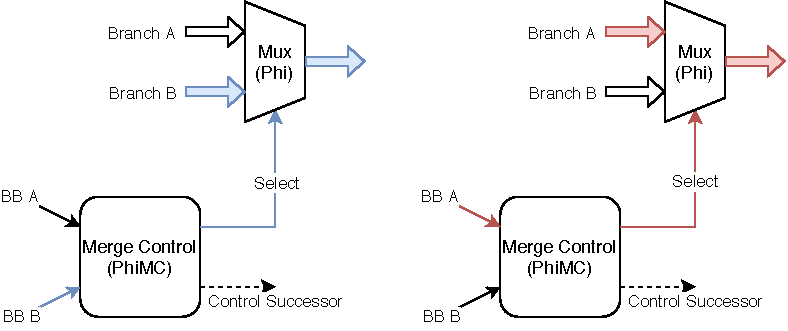
\includegraphics[width=0.8\textwidth]{Images/mux_mc_exp.pdf}
    \caption{Diagram of the \code{mux} and \code{merge\_ctrl} component relation. The select signal is generated from the control flow input.}
    \label{fig:mux_mc}
\end{figure}

The multiplexer or \code{mux} components function the same as their hardware counterparts. Figure \ref{fig:mux_mc} shows the connection between basic blocks and the control of the \code{mux} components. The \code{merge\_ctrl} receives the valid signal from the control components of the predecessor basic blocks, this signal is converted into a select signal to choose the appropriate branch attached to the \code{mux} inputs. The \code{mux} then allows the data from that branch through to the output. The difficulty is determining the basic block control signal for the data branches. This could be gathered by iterating over the branches in predecessor blocks but it was simpler to add this information when constructing the \code{mux} components. The basic block numbers are stored in a separate array, the index of the array corresponds to the branch predecessors. Each basic block has a maximum of one \code{merge\_ctrl}, the pass iterates through and connects the output of the component to the \code{mux} select line inputs. A check is performed to make sure that the control branch order matches the data branch order, any differences are corrected.


\iffalse	
implementing control flow
	first iteration only worked by connecting the branches instantiated in the initial conversion
	testing with more complex functions revealed the issue of nothing (null) nodes
	nothing nodes were a simple fix, when doing the initial conversion, they are treated like a goto, that is, a control branch with a constant input
	
	next issue was how link up muxes, separate fields were added to the mux and merg ctrl
	iterate through the stmts in each bb, only one merge ctrl - greater than one input
	for every mux found, iterate through the bb info - verify length, make sure the preds match the order of the branches into the merge ctrl
	
	final ctrl issue - initial assumption was about gotoifnot, true branch is fall throguh, otherwise false
	led to issues when looping as the true branch was not just fall through, it was a bb much further back - resolve this, if there is only one successor - default to true
	
next passes add forks since standard operations cannont have more than one successor
	sinks to tie off any 
	sources required to be at the head of the constants
	maybe explain petri nets here?

\fi

\begin{figure}[htb!]
    \centering
    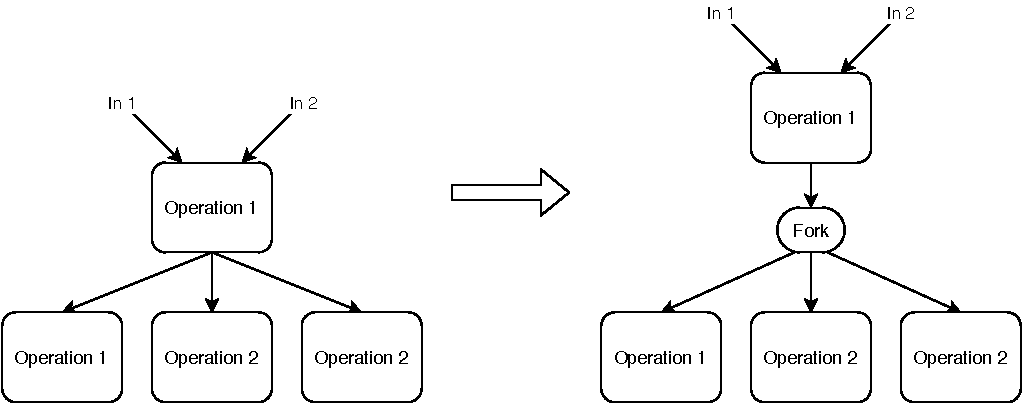
\includegraphics[width=0.9\textwidth]{Images/fork_pass.pdf}
    \caption{Visual representation of the \code{fork} implementation pass.}
    \label{fig:fork_pass}
\end{figure}

\subsection{Final Structural Passes}
The elastic components in the dynamatic library follow have a predefined input/output structure. The components are designed to be with operations like multiply or divide having two inputs and one output. Results of these operations are likely to act as inputs to multiple components. To facilitate the splitting of data flow, the fork pass was implemented to add an additional component between the operation outputs as in Figure \ref{fig:fork_pass}. The \code{fork} component splits the valid/ready signals over the successor components so that each can operate and the data can flow through subsequent operations.

\begin{figure}[htb!]
    \centering
    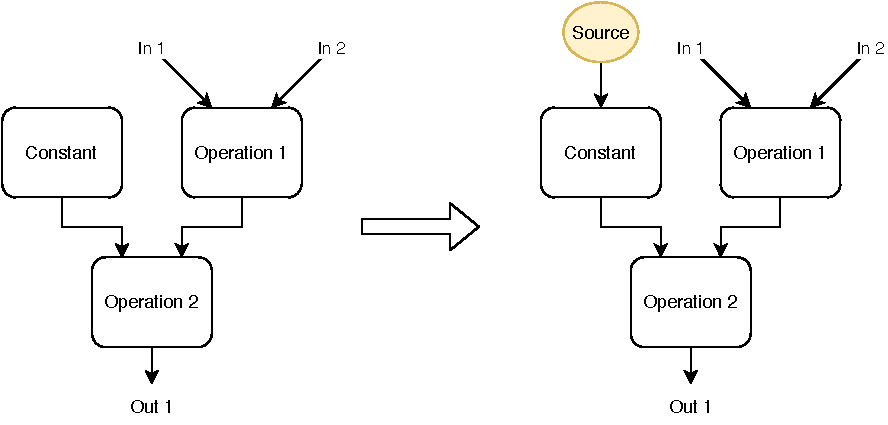
\includegraphics[width=\textwidth]{Images/source_pass.pdf}
    \caption{Visual representation of the \code{source} implementation pass.}
    \label{fig:source_pass}
\end{figure}

The two remaining components to be added are the source and sink. These components are required because the elastic circuit communication relies on the petri-net model \cite{petri}. The valid/ready signals used for controlling data flow act as the tokens passing between individual components. When a token is received (a valid signal asserted) then the component can perform it's operation, providing it is ready to do so. All the elastic circuits have a \code{start} at the head of the control flow. The token is passed from this component to all other components except for constant values. These components require their own tokens so that the flow continues. \code{source} components are attached as input to the constants as in Figure \ref{fig:source_pass}. These continuously assert valid so that the constant has a continual amount of tokens to allow the constant data to flow to subsequent components. \code{sink} components are the opposite of \code{source} and consume tokens. They have a constantly asserted ready signal so accept all incoming valid signals. This allows the elastic circuit to be tied off where there are no data flow connections. Figure \ref{fig:sink_pass} shows the \code{sink} node being attached to the unused connection of a branch with a constant-driven select line.

\begin{figure}[htb!]
    \centering
    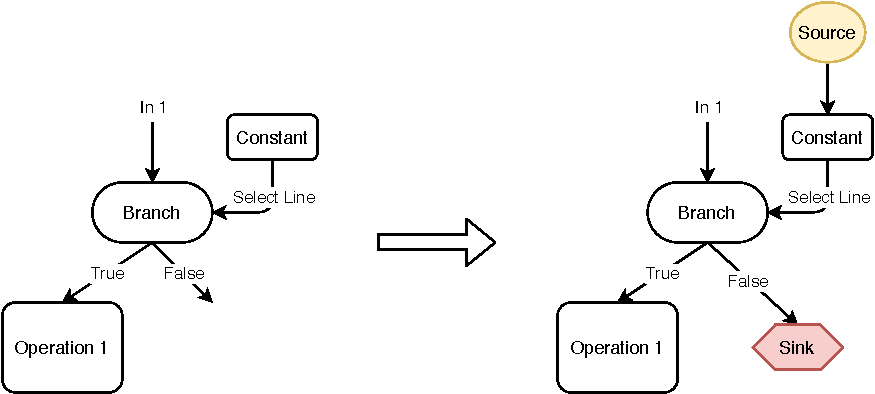
\includegraphics[width=\textwidth]{Images/sink_pass.pdf}
    \caption{Visual representation of the \code{sink} implementation pass.}
    \label{fig:sink_pass}
\end{figure}

\subsubsection{Cycles}
The VHDL components consist primarily of combinatorial logic statements meaning that cycles within the circuit cause a deadlock. This occurs at the entry point to the cycle. The cycle will start with a \code{mux} or merging component with at least two predecessor basic blocks. The predecessor block will be the entry to the loop. The second will be an eventual successor to the current block, forming the loop. For the data to flow through the merging component, it's successor component must be ready. It follows that all successors must be ready for data to flow. Since there is an eventual connection from the merging component successors round the cycle to be a predecessor to the merging component, it is not possible for the components to achieve a ready state so data cannot flow through the cycle, hence deadlock. The dynamatics library includes buffer components as one of the fundamental elastic components. Buffers introduce an always ready component into the cycle, breaking the deadlock. Since the logic is primarily combinatorial, the buffer would cause an unstable state for the circuit so the buffer registers the input and result of the loop is evaluated at the next clock cycle without affecting the functional correctness.

The simple method to introduce buffers in the dynamatic library searches for every data merge node with two or more inputs and adds a buffer in case there is a cycle. This works to make sure each cycle has a buffer but may add unnecessary buffers such as in the event a program has no cycle. At this stage in the development of the flow this is not needed so an alternative function was implemented to add buffers at the heads of cycles. With the components alone, it is difficult to determine the cycles within a program. The cycle pass instead uses the CFG to derive the cycles in the program by converting the CFG to the Lightgraph \cite{julia_lightgrph} format and using the \code{simple\_cycles} method to determine the paths in the CFG that form cycles. Each path is returned and the heads of these basic block paths are accumulated. Finally, the pass iterates through the components and adds a buffer after each \code{mux} and \code{merge\_ctrl} component in the corresponding basic blocks as in Figure \ref{fig:buffer_pass}.

\begin{figure}[htb!]
    \centering
    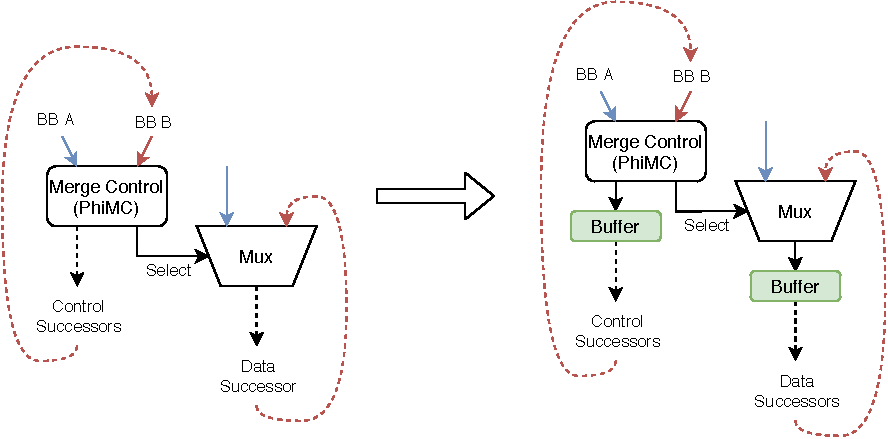
\includegraphics[width=\textwidth]{Images/cycle_pass.pdf}
    \caption{Demostrates the insertion points of \code{buffer} components in a cyclic program.}
    \label{fig:buffer_pass}
\end{figure}

\iffalse
components are primarily combinatorial logic
	cycles withtin the generated circuit cause deadlock as no ready signal available form down stream because no valid signal from upstream
	simple algorithm is naive. since all loops must have phi nodes as a SSA rule, add buffer circuitry in these basic blocks. The buffer has no backpressure in that the valid signal is always high
	the buffer introduces a register to the chain, so that the information is passed through on the next cycle the pred is ready
	
this is great but since every phi gets a buffer, it introduces more than is necessary such as when there are no loops
	at this stage you dont want to add them for acyclic functions	
	different version of the function converts the CFG into a directed light graph
	using lightgraph method - simple\_ccyels
		determines all the cycles for the function 
		pick the lowest bb in the cycle
		add to list - using union so not doubled up
		iterate through bbs and add buffers after the merge control and muxs in the corresponding bb
		this provides the minimum buffers for given function
\fi


\iffalse
Implementation
give details about the code
discuss important and interesting aspects
anything that was surprising or difficult
State clearly what is left out
dont just chuck in code
	make sure it is relevant, might be better to chuck in algorithms
	illustrate algo flow
	highlight and optimisation
	demonstrate data structure interactions
any screenshots should be useful, not just proof a tool was run
	eg waveforms or statemachines
best to focus on conceptual logical design and go into detail on interesting parts
often times diagrams of hw or code interaction better convey code info
include code listings in appendix, links to github repos
\fi